\chapter{浓度与稀释}\label{ch:g10:concentration-and-dilution}

医院里的输液袋悬挂在病床上方。袋上的标签写着“0.9 \%
氯化钠”：盐溶于水，仅此而已。然而数字 0.9 并非细节。
盐太少，患者的血细胞会吸水膨胀；
盐太多，则会皱缩。溶液不能仅由其成分描述，
还须说明每单位体积中含有多少\omterm{def:g6:solutions-and-solubility:solute}{溶质}，
即其浓度。本章将测量浓度、配制浓度准确的溶液，
并对溶液进行\omterm{def:g10:concentration-and-dilution:dilution}{稀释}。

\begin{recall}
溶液由\omterm{def:g6:solutions-and-solubility:solute}{溶剂}与一种或多种\omterm{def:g2:mixing-and-dissolving:dissolve}{溶解}的\omterm{def:g6:solutions-and-solubility:solute}{溶质}组成；\omterm{def:g6:solutions-and-solubility:solubility}{溶解度}是
一定量\omterm{def:g6:solutions-and-solubility:solute}{溶剂}能\omterm{def:g2:mixing-and-dissolving:dissolve}{溶解}的\omterm{def:g6:solutions-and-solubility:solute}{溶质}的最大质量
（见\cref{ch:g6:solutions-and-solubility}）。某物种的\omterm{def:g10:the-mole:amount}{物质的量}
为 $n = m/M$，单位为\omterm{def:g10:the-mole:amount}{摩尔}（见\cref{ch:g10:the-mole}）。
\end{recall}

\begin{omfigure}
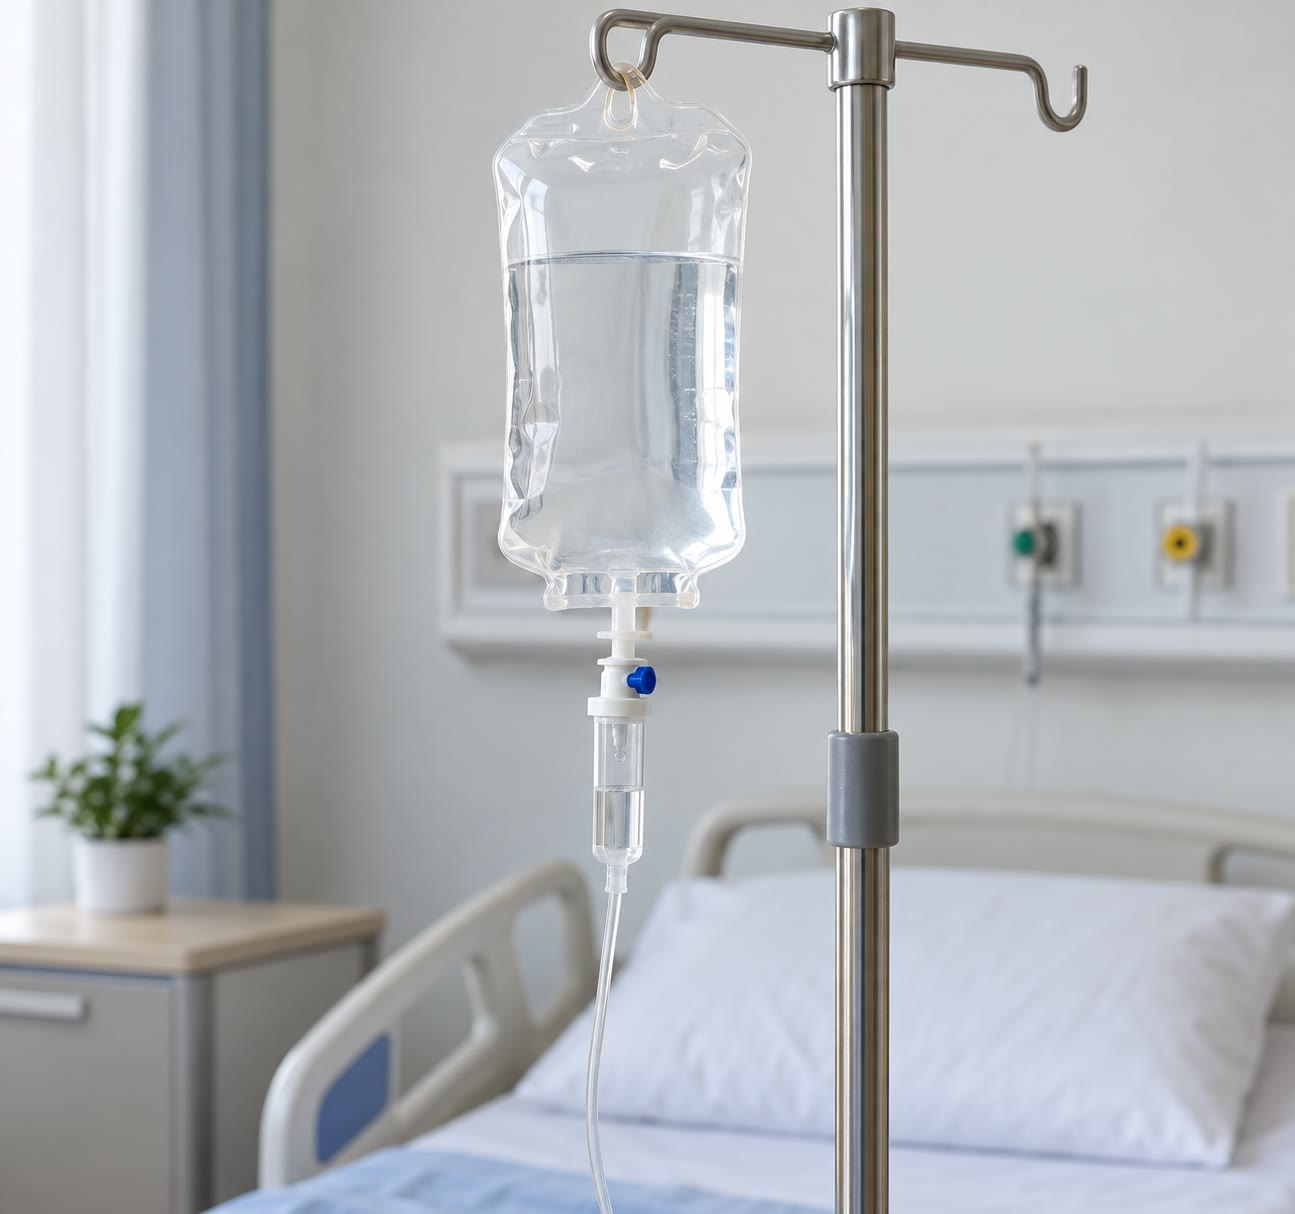
\includegraphics[width=0.42\linewidth]{images/book1/ai/g10-drip-bag.jpg}

{\small 盐溶液输液袋：浓度必须准确。}
\end{omfigure}

\section{质量浓度}

\begin{definition}[质量浓度]\label{def:g10:concentration-and-dilution:mass-concentration}
溶液中\omterm{def:g6:solutions-and-solubility:solute}{溶质}的\emph{质量浓度}\index{质量浓度} $C_m$
为单位体积溶液中所\omterm{def:g2:mixing-and-dissolving:dissolve}{溶解}\omterm{def:g6:solutions-and-solubility:solute}{溶质}的质量：
\[
  C_m = \frac{m_{\text{溶质}}}{V_{\text{溶液}}},
\]
单位为克每升（\si{g/L}）。
\end{definition}

\begin{example}[糖水]\label{ex:g10:concentration-and-dilution:sugar}
将 \qty{20}{g} 糖溶于水，并配成
\qty{0.50}{L} 溶液。其中糖的\omterm{def:g10:concentration-and-dilution:mass-concentration}{质量浓度}为
$C_m = \qty{20}{g} / \qty{0.50}{L} = \qty{40}{g/L}$。溶液的任一部分
浓度相同：\qty{0.20}{L} 的一杯中含糖
$\qty{40}{g/L} \times \qty{0.20}{L} = \qty{8.0}{g}$。
\end{example}


\begin{remark}[体积指溶液的体积]\label{rem:g10:concentration-and-dilution:volume}
$C_m$ 中的体积是整个溶液的体积，而非
所加入水的体积：\omterm{def:g2:mixing-and-dissolving:dissolve}{溶解}\omterm{def:g6:solutions-and-solubility:solute}{溶质}会使体积略有改变。因此
溶液总要\emph{配成}已知的最终体积，
在带有相应刻度的专用容量瓶中进行。
\end{remark}

\begin{remark}[浓度不等于溶解度]\label{rem:g10:concentration-and-dilution:not-solubility}
% ledger: sol:NaCl, saline:NaCl
\omterm{def:g6:solutions-and-solubility:solute}{溶质}的\omterm{def:g6:solutions-and-solubility:solubility}{溶解度}是它所能达到的\emph{最大}浓度；
溶液的浓度可以从零到该最大值之间的任意值。氯化钠
在 \qty{25}{\celsius} 时，每千克水中最多可\omterm{def:g2:mixing-and-dissolving:dissolve}{溶解}约 \qty{360}{g}；
而输液袋中每升仅含 \qty{9}{g}，
远未达到饱和。
\end{remark}

\begin{remark}[标签上的百分数]\label{rem:g10:concentration-and-dilution:percent}
% ledger: saline:NaCl
在医药和食品标签上，固体溶于水时所标的“0.9 \%”
通常表示每 \qty{100}{mL} 溶液中含 \qty{0.9}{g} \omterm{def:g6:solutions-and-solubility:solute}{溶质}。以
克每升计，数值为其十倍：输液袋中含氯化钠
\qty{9.0}{g/L}。
\end{remark}

\section{物质的量浓度}

\begin{definition}[物质的量浓度]\label{def:g10:concentration-and-dilution:molar-concentration}
溶液中\omterm{def:g6:solutions-and-solubility:solute}{溶质}的\emph{物质的量浓度}\index{物质的量浓度} $c$
为单位体积溶液中所\omterm{def:g2:mixing-and-dissolving:dissolve}{溶解}\omterm{def:g6:solutions-and-solubility:solute}{溶质}的
\omterm{def:g10:the-mole:amount}{物质的量}：
\[
  c = \frac{n_{\text{溶质}}}{V_{\text{溶液}}},
\]
单位为\omterm{def:g10:the-mole:amount}{摩尔}每升（\si{mol/L}）。
\end{definition}

\begin{proposition}[两种浓度之间的换算]\label{prop:g10:concentration-and-dilution:link}
对于\omterm{def:g10:the-mole:molar-mass}{摩尔质量}为 $M$ 的\omterm{def:g6:solutions-and-solubility:solute}{溶质}，
\[
  C_m = c \times M .
\]
\end{proposition}

\begin{proof}
$C_m = m / V = (n \times M) / V = (n / V) \times M = c \times M$.
\end{proof}

\begin{example}[以摩尔计的输液袋]\label{ex:g10:concentration-and-dilution:drip}
% ledger: saline:NaCl, saline:Na, aw:Na, aw:Cl
输液袋中含氯化钠 \qty{9.0}{g/L}，其\omterm{def:g10:the-mole:molar-mass}{摩尔质量}为
\qty{58.5}{g/mol}。其\omterm{def:g10:concentration-and-dilution:molar-concentration}{物质的量浓度}为
\[
  c = \frac{C_m}{M} = \frac{\qty{9.0}{g/L}}{\qty{58.5}{g/mol}}
    = \qty{0.154}{mol/L}.
\]
厂家标签以另一种方式给出同一数值：每升溶液中
含钠\omterm{def:g9:ions:ion}{离子} 154 毫\omterm{def:g10:the-mole:amount}{摩尔}。
\end{example}

\begin{remark}[溶液中的离子]\label{rem:g10:concentration-and-dilution:ions}
氯化钠以独立的\omterm{def:g9:ions:ion}{离子} \ce{Na+} 和 \ce{Cl-} \omterm{def:g2:mixing-and-dissolving:dissolve}{溶解}
（见\cref{ch:g9:ions}）：浓度为 \qty{0.154}{mol/L} 的氯化钠溶液中，
含钠\omterm{def:g9:ions:ion}{离子} \qty{0.154}{mol/L}，
含氯\omterm{def:g9:ions:ion}{离子} \qty{0.154}{mol/L}。\omterm{def:g9:ions:ion}{离子}型固体在水中如何解离，
将在后面章节中讨论。
\end{remark}

\begin{omfigure}
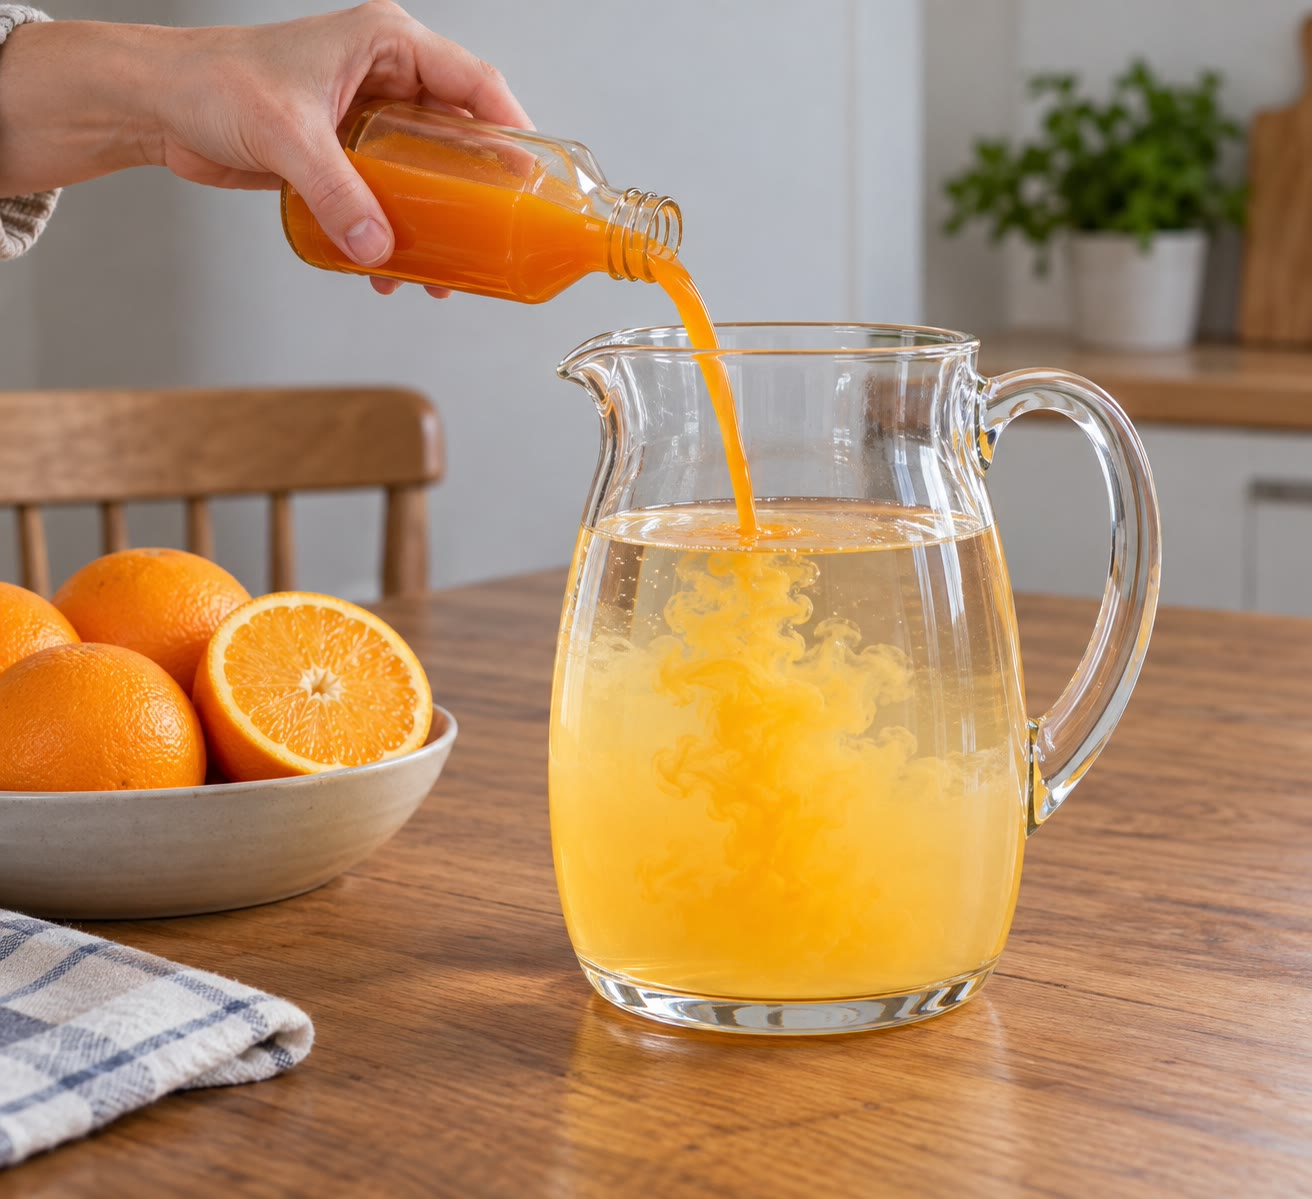
\includegraphics[width=0.45\linewidth]{images/book1/ai/g10-squash-jug.jpg}

{\small 瓶装果汁在壶中加水\omterm{def:g10:concentration-and-dilution:dilution}{稀释}：饮料中果汁糖浆的量不变，
但体积更大。}
\end{omfigure}

\section{通过溶解配制溶液}

\begin{method}[溶解固体配制溶液]\label{met:g10:concentration-and-dilution:dissolving}
欲配制体积为 $V$、\omterm{def:g10:concentration-and-dilution:molar-concentration}{物质的量浓度}为 $c$ 的溶液：
\begin{enumerate}
  \item 计算所需\omterm{def:g10:the-mole:amount}{物质的量} $n = c \times V$，
        以及需称取的质量 $m = n \times M$。
  \item 用天平在小表面皿中称取该质量的固体。
  \item 通过漏斗将固体倒入体积为
        $V$ 的容量瓶中；用\omterm{def:g10:chemical-species:distillation}{蒸馏}水冲洗表面皿和漏斗，
        使洗液全部进入容量瓶，确保固体无损失。
  \item 加入\omterm{def:g10:chemical-species:distillation}{蒸馏}水至容量瓶约半满，
        摇动直至固体全部\omterm{def:g2:mixing-and-dissolving:dissolve}{溶解}。
  \item 加\omterm{def:g10:chemical-species:distillation}{蒸馏}水至刻度线，最后几滴用滴管加入；
        塞好瓶塞，上下颠倒数次使其混匀。
\end{enumerate}
\end{method}

\begin{omfigure}
\begin{tikzpicture}[font=\small, scale=1.05]
  % 1. weigh
  \pic[transform shape] at (0,0) {balance};
  \fill[black!8, draw=black!55] (-0.45,0.8) -- (0.45,0.8) -- (0.38,0.98)
    -- (-0.38,0.98) -- cycle;
  \fill[white, draw=black!40] (-0.25,0.98) .. controls (-0.1,1.15) and
    (0.1,1.15) .. (0.25,0.98) -- cycle;
  \node[align=center, anchor=north] at (0,-0.2) {1. 称量 \\ 固体};
  % 2. transfer through a funnel
  \pic[transform shape] at (3.2,0) {volflask={0.08}{omWater}};
  \pic[transform shape] at (3.2,3.0) {funnel};
  \draw[omProp, thick, -{Stealth}] (2.4,5.0) -- (2.85,4.65);
  \node[align=center, anchor=north] at (3.2,-0.2) {2. 转移，\\ 冲洗};
  % 3. half full, swirl
  \pic[transform shape] at (6.4,0) {volflask={0.45}{omWater}};
  \draw[omProp, thick, -{Stealth}] (5.55,0.5) arc[start angle=200,
    end angle=340, x radius=0.9, y radius=0.3];
  \node[align=center, anchor=north] at (6.4,-0.2) {3. 半满：\\ 摇动溶解};
  % 4. to the mark
  \pic[transform shape] at (9.6,0) {volflask={1}{omWater}};
  \fill[black!45] (9.43,3.6) rectangle (9.77,3.85);
  \draw[omDef, thick, <-] (9.82,2.9) -- (10.6,3.3) node[right] {刻度线};
  \node[align=center, anchor=north] at (9.6,-0.2) {4. 加至刻度，\\
    塞好，混匀};
\end{tikzpicture}

{\small 通过\omterm{def:g2:mixing-and-dissolving:dissolve}{溶解}固体配制溶液：称量、转移、\omterm{def:g2:mixing-and-dissolving:dissolve}{溶解}，
然后加水至容量瓶的刻度线。}
\end{omfigure}

\begin{inthelab}[定容]
容量瓶的刻度线是瓶颈上的一圈标记。细玻璃管中的水
面并不平整，液面中央向下凹，形成弯月面。
当眼睛与刻度线平齐，弯月面的\emph{最低点}恰好与刻度线相切时，
容量瓶即已装满，此时前后两侧的刻度环看起来连成一条线。
从上方或下方观察，
液面看起来可能正好，
实际却未必如此。
\end{inthelab}

\begin{omfigure}
\begin{tikzpicture}[font=\small]
  \newcommand{\neck}[2]{% x, meniscus bottom height
    \fill[omWater] (#1-0.5,0) -- (#1-0.5,{#2+0.25}) .. controls
      (#1-0.25,#2) and (#1+0.25,#2) .. (#1+0.5,{#2+0.25}) -- (#1+0.5,0) -- cycle;
    \draw[black!60, line width=0.8pt] (#1-0.5,0) -- (#1-0.5,3);
    \draw[black!60, line width=0.8pt] (#1+0.5,0) -- (#1+0.5,3);
    \draw[omDef, line width=0.9pt] (#1-0.5,1.5) -- (#1+0.5,1.5);
    \draw[black!50] (#1-0.5,{#2+0.25}) .. controls (#1-0.25,#2) and
      (#1+0.25,#2) .. (#1+0.5,{#2+0.25});}
  \newcommand{\eye}[2]{% x, y: an eye looking to the right
    \draw[black!70] (#1-0.25,#2) .. controls (#1-0.1,#2+0.18) and
      (#1+0.1,#2+0.18) .. (#1+0.2,#2) .. controls (#1+0.1,#2-0.18) and
      (#1-0.1,#2-0.18) .. (#1-0.25,#2);
    \fill[black!70] (#1+0.05,#2) circle (0.06);}
  % right
  \neck{1.5}{1.5}
  \eye{-0.4}{1.5}
  \draw[dashed, black!50] (-0.1,1.5) -- (2.4,1.5);
  \node[align=center] at (1.5,-0.55) {正确：视线平齐，\\ 弯月面底部在刻度线};
  % too high
  \neck{6}{1.85}
  \eye{4.1}{1.85}
  \draw[dashed, black!50] (4.4,1.85) -- (6.9,1.85);
  \node[align=center] at (6,-0.55) {水过多：\\ 弯月面在上方};
  % too low
  \neck{10.5}{0.85}
  \eye{8.6}{0.85}
  \draw[dashed, black!50] (8.9,0.85) -- (11.4,0.85);
  \node[align=center] at (10.5,-0.55) {水过少：\\ 弯月面在下方};
\end{tikzpicture}

{\small 容量瓶瓶颈放大图，图中为从弯月面高度处观察的视线，
图中蓝线为刻度线。
只有左侧的容量瓶液面正确。}
\end{omfigure}

\section{稀释}

\begin{definition}[稀释、母液、稀释倍数]\label{def:g10:concentration-and-dilution:dilution}
\emph{稀释}\index{稀释}是降低溶液浓度的过程，
即加入\omterm{def:g6:solutions-and-solubility:solute}{溶剂}。开始时取用的浓溶液称为
\emph{母液}\index{母液}。
\emph{稀释倍数}\index{稀释倍数} $F$ 为母液浓度与
稀释后溶液浓度之比：
\[
  F = \frac{c_{\text{母液}}}{c_{\text{稀释后}}} .
\]
\end{definition}

\begin{proposition}[溶质的量保持不变]\label{prop:g10:concentration-and-dilution:kept}
\omterm{def:g10:concentration-and-dilution:dilution}{稀释}过程中，\omterm{def:g6:solutions-and-solubility:solute}{溶质}的量保持不变：若
取体积为 $V_0$、浓度为 $c_0$ 的\omterm{def:g10:concentration-and-dilution:dilution}{母液}，\omterm{def:g10:concentration-and-dilution:dilution}{稀释}至
体积 $V_1$，则\omterm{def:g10:concentration-and-dilution:dilution}{稀释}后溶液的浓度为 $c_1$，由下式给出：
\[
  c_0 \times V_0 = c_1 \times V_1,
  \qquad\text{故}\qquad
  F = \frac{c_0}{c_1} = \frac{V_1}{V_0} .
\]
对\omterm{def:g10:concentration-and-dilution:mass-concentration}{质量浓度}同样成立。
\end{proposition}

\begin{proof}
只加入\omterm{def:g6:solutions-and-solubility:solute}{溶剂}：取出的体积为 $V_0$ 的\omterm{def:g6:solutions-and-solubility:solute}{溶质}，
其量为 $c_0 V_0$，全部位于终体积 $V_1$ 中，
其\omterm{def:g10:the-mole:amount}{物质的量}即为 $c_1 V_1$。
\end{proof}


\begin{method}[用稀释法配制溶液]\label{met:g10:concentration-and-dilution:diluting}
欲配制体积为 $V_1$、浓度为 $c_1$ 的溶液，
所用\omterm{def:g10:concentration-and-dilution:dilution}{母液}的浓度为 $c_0$：
\begin{enumerate}
  \item 计算所需\omterm{def:g10:concentration-and-dilution:dilution}{母液}的体积，
        $V_0 = c_1 V_1 / c_0$（即 $V_1 / F$）。
  \item 将少量\omterm{def:g10:concentration-and-dilution:dilution}{母液}倒入干净的烧杯中（切勿直接从\omterm{def:g7:identifying-substances:characteristic-test}{试剂}瓶中移取），
        再用容量移液管准确移取 $V_0$ 体积的\omterm{def:g10:concentration-and-dilution:dilution}{母液}，
        吸至刻度线。
  \item 将移液管中的\omterm{def:g10:concentration-and-dilution:dilution}{母液}全部放入容积为 $V_1$ 的容量瓶中。
  \item 加\omterm{def:g10:chemical-species:distillation}{蒸馏}水至刻度线，塞紧瓶塞并混匀。
\end{enumerate}
\end{method}

\begin{example}[一次十倍稀释]\label{ex:g10:concentration-and-dilution:tenfold}
某硫酸铜\omterm{def:g10:concentration-and-dilution:dilution}{母液}，其 $c_0 = \qty{0.10}{mol/L}$；
需配制 \qty{100.0}{mL} 浓度为 $c_1 = \qty{0.010}{mol/L}$ 的溶液。\omterm{def:g10:concentration-and-dilution:dilution}{稀释
倍数}为 $F = 0.10 / 0.010 = 10$，故 $V_0 = \qty{100.0}{mL} / 10 =
\qty{10.0}{mL}$：需用 \qty{10.0}{mL} 移液管和 \qty{100.0}{mL} 容量瓶。
\end{example}

\begin{omfigure}
\begin{tikzpicture}[font=\small, scale=0.85]
  % 1. take the stock with a pipette
  \pic[transform shape] at (0,0) {beaker={0.6}{cyan!70!blue!55}};
  \pic[transform shape] at (0,0.2) {pipette={1}{cyan!70!blue!55}};
  \node[align=center, anchor=north] at (0,-0.2) {1. 移取 $V_0$\\ 母液};
  \draw[omProp, very thick, -{Stealth}] (1.3,2.6) -- (2.6,2.6);
  % 2. empty it into the flask
  \pic[transform shape] at (4,0) {volflask={0.22}{cyan!70!blue!55}};
  \pic[transform shape] at (4,2.6) {pipette={0.12}{cyan!70!blue!55}};
  \node[align=center, anchor=north] at (4,-0.2) {2. 放入 \\ 容量瓶};
  \draw[omProp, very thick, -{Stealth}] (5.3,2.6) -- (6.6,2.6);
  % 3. water to the mark
  \pic[transform shape] at (8,0) {volflask={1}{cyan!70!blue!14}};
  \draw[omDef, thick, <-] (8.2,2.9) -- (9.1,3.4) node[right] {刻度线};
  \node[align=center, anchor=north] at (8,-0.2) {3. 加水至刻度线：\\
    体积 $V_1$};
\end{tikzpicture}

{\small \omterm{def:g10:concentration-and-dilution:dilution}{稀释}：用移液管量取体积为 $V_0$ 的\omterm{def:g10:concentration-and-dilution:dilution}{母液}，
在容量瓶中定容至 $V_1$。颜色变浅的
倍数即\omterm{def:g10:concentration-and-dilution:dilution}{稀释倍数} $V_1 / V_0$。}
\end{omfigure}

\section{标准色阶}

\begin{definition}[标准溶液、标准色阶]\label{def:g10:concentration-and-dilution:standard}
浓度精确已知的溶液称为
\emph{标准溶液}\index{标准溶液}。同一\omterm{def:g6:solutions-and-solubility:solute}{溶质}、浓度递增的
一系列标准溶液，称为\emph{标准色阶}\index{标准色阶}，
通常由同一\omterm{def:g10:concentration-and-dilution:dilution}{母液}\omterm{def:g10:concentration-and-dilution:dilution}{稀释}而得；
将未知溶液与之比较，
即可估计未知溶液的浓度。
\end{definition}

\begin{example}[蓝色色阶]\label{ex:g10:concentration-and-dilution:scale}
取浓度为 \qty{0.20}{mol/L} 的硫酸铜\omterm{def:g10:concentration-and-dilution:dilution}{母液}，
配制 6 份\omterm{def:g10:concentration-and-dilution:standard}{标准溶液}，浓度分别为 0.02、0.04、0.06、0.08、0.10 和
\qty{0.12}{mol/L}，各装入相同的试管，并装至相同高度。
另取一份浓度未知的溶液，装入同类试管中，颜色
比 \qty{0.06}{mol/L} 的试管深，比
\qty{0.08}{mol/L} 的试管浅，故其浓度介于两者之间，约为
\qty{0.07}{mol/L}。
\end{example}

\begin{omfigure}
\begin{tikzpicture}[font=\small]
  \foreach \i/\c/\p in {0/0.02/8, 1/0.04/16, 2/0.06/24, 3/0.08/32,
                        4/0.10/40, 5/0.12/48} {
    \pic at (1.2*\i,0) {testtube={0.75}{cyan!70!blue!\p}};
    \node[anchor=north] at (1.2*\i,-0.15) {\c};
  }
  \pic at (8.4,0) {testtube={0.75}{cyan!70!blue!28}};
  \node[anchor=north] at (8.4,-0.15) {?};
  \draw[black!40] (7.55,-0.6) -- (7.55,3.2);
  \node[anchor=north] at (3,-0.7) {浓度 (\si{mol/L})};
  \node[anchor=north] at (8.4,-0.7) {未知};
\end{tikzpicture}

{\small 硫酸铜溶液的\omterm{def:g10:concentration-and-dilution:standard}{标准色阶}与一份未知溶液。
未知溶液位于第 3 支与第 4 支试管之间。}
\end{omfigure}

\begin{safety}{\ghs[0.82cm]{GHS05}\ghs[0.82cm]{GHS07}\ghs[0.82cm]{GHS09}}
% ledger: ghs:CuSO4
硫酸铜溶液：吞食有害，刺激皮肤，
会损伤眼睛，对水生生物毒性极强。须佩戴护目镜与手套；
用过的溶液须收集后统一处理，切勿倒入水槽。
\end{safety}

\begin{remark}[眼睛的局限]\label{rem:g10:concentration-and-dilution:eye}
眼睛只能判断“介于这两支试管之间”。要更精细地从溶液颜色测定浓度，
化学家测量的是溶液吸收了多少光；
后面的章节会专门讲这一方法。
\end{remark}

\section{练习}

\begin{exercise}[$\star$]\label{exo:g10:concentration-and-dilution:1}
将\qty{5.0}{g}糖\omterm{def:g2:mixing-and-dissolving:dissolve}{溶解}，配成\qty{250}{mL}溶液。
计算该糖溶液的\omterm{def:g10:concentration-and-dilution:mass-concentration}{质量浓度}，单位为克每升。
\end{exercise}

\begin{exercise}[$\star$]\label{exo:g10:concentration-and-dilution:2}
某\qty{200}{mL}溶液中含有\qty{0.050}{mol}葡萄糖。
计算其\omterm{def:g10:concentration-and-dilution:molar-concentration}{物质的量浓度}。
\end{exercise}

\begin{exercise}[$\star$]\label{exo:g10:concentration-and-dilution:3}
需称取多少质量的无水硫酸铜\ce{CuSO4}，以配制
\qty{100.0}{mL}浓度为\qty{0.10}{mol/L}的溶液？
\end{exercise}

\begin{exercise}[$\star$]\label{exo:g10:concentration-and-dilution:4}
将\qty{1.0}{mol/L}的\omterm{def:g10:concentration-and-dilution:dilution}{母液}\omterm{def:g10:concentration-and-dilution:dilution}{稀释}至\qty{0.050}{mol/L}。
求\omterm{def:g10:concentration-and-dilution:dilution}{稀释倍数}。配制
\qty{100.0}{mL}\omterm{def:g10:concentration-and-dilution:dilution}{稀释}后的溶液，需要多少体积的\omterm{def:g10:concentration-and-dilution:dilution}{母液}？
\end{exercise}

\begin{exercise}[$\star$]\label{exo:g10:concentration-and-dilution:5}
氯化钠溶液的\omterm{def:g10:concentration-and-dilution:molar-concentration}{物质的量浓度}为
\qty{0.10}{mol/L}，求其\omterm{def:g10:concentration-and-dilution:mass-concentration}{质量浓度}。
\end{exercise}

\begin{exercise}[$\star\star$]\label{exo:g10:concentration-and-dilution:6}
需取多少体积浓度为\qty{0.50}{mol/L}的\omterm{def:g10:concentration-and-dilution:dilution}{母液}，以
配制\qty{250.0}{mL}浓度为\qty{0.020}{mol/L}的溶液？请指出所用的两种
玻璃仪器。
\end{exercise}

\begin{exercise}[$\star\star$]\label{exo:g10:concentration-and-dilution:7}
为什么配制准确浓度的溶液要用容量瓶，
而不用带刻度的烧杯？为什么量取\omterm{def:g10:concentration-and-dilution:dilution}{母液}时
要用移液管，而不用
量筒？
\end{exercise}

\begin{exercise}[$\star\star$]\label{exo:g10:concentration-and-dilution:8}
观察硫酸铜的\omterm{def:g10:concentration-and-dilution:standard}{标准色阶}。另一未知溶液
颜色比\qty{0.04}{mol/L}的试管浅，但比
\qty{0.02}{mol/L}的试管深。估算其浓度。如何改进\omterm{def:g10:concentration-and-dilution:standard}{标准色阶}，
才能更精确地估算？
\end{exercise}

\begin{exercise}[$\star\star$]\label{exo:g10:concentration-and-dilution:9}
某输液用葡萄糖溶液中含有\qty{50}{g/L}的葡萄糖，
\ce{C6H12O6}，计算其\omterm{def:g10:concentration-and-dilution:molar-concentration}{物质的量浓度}。
\end{exercise}

\begin{exercise}[$\star\star$]\label{exo:g10:concentration-and-dilution:10}
制得糖浆，方法是将\qty{342}{g}蔗糖\ce{C12H22O11}\omterm{def:g2:mixing-and-dissolving:dissolve}{溶解}，
配成\qty{1.00}{L}溶液。计算其\omterm{def:g10:concentration-and-dilution:molar-concentration}{物质的量浓度}，随后\omterm{def:g10:concentration-and-dilution:dilution}{稀释}十倍，
求\qty{20}{mL}\omterm{def:g10:concentration-and-dilution:dilution}{稀释}后糖浆中
所含蔗糖的质量。
\end{exercise}

\begin{exercise}[$\star\star$]\label{exo:g10:concentration-and-dilution:11}
某溶液的\omterm{def:g10:concentration-and-dilution:mass-concentration}{质量浓度}为\qty{12}{g/L}。求下列情形下其浓度：
(a) 加水使体积加倍后；(b) \omterm{def:g3:separating-mixtures:evaporate}{蒸发}掉一半的水，
且\omterm{def:g6:solutions-and-solubility:solute}{溶质}仍全部\omterm{def:g2:mixing-and-dissolving:dissolve}{溶解}后，
其浓度各为多少？
\end{exercise}

\begin{exercise}[$\star\star\star$]\label{exo:g10:concentration-and-dilution:12}
将浓度为\qty{0.10}{mol/L}的溶液\omterm{def:g10:concentration-and-dilution:dilution}{稀释}十倍，
所得溶液再\omterm{def:g10:concentration-and-dilution:dilution}{稀释}十倍，然后再\omterm{def:g10:concentration-and-dilution:dilution}{稀释}一次。
\begin{enumerate}
  \item 最终浓度是多少？
  \item 为什么要分三步进行，而不是一次\omterm{def:g10:concentration-and-dilution:dilution}{稀释}
        1000 倍？（请考虑所需玻璃仪器的体积。）
\end{enumerate}
\end{exercise}

\begin{exercise}[$\star\star\star$]\label{exo:g10:concentration-and-dilution:13}
将\qty{11.1}{g}氯化钙\ce{CaCl2}\omterm{def:g2:mixing-and-dissolving:dissolve}{溶解}，配成
\qty{500.0}{mL}溶液。在水中，该固体会电离为钙
\omterm{def:g9:ions:ion}{离子}\ce{Ca^2+}和氯\omterm{def:g9:ions:ion}{离子}\ce{Cl-}。
\begin{enumerate}
  \item 计算所\omterm{def:g2:mixing-and-dissolving:dissolve}{溶解}氯化钙的\omterm{def:g10:concentration-and-dilution:molar-concentration}{物质的量浓度}。
  \item 推出溶液中钙\omterm{def:g9:ions:ion}{离子}和
        氯\omterm{def:g9:ions:ion}{离子}的\omterm{def:g10:concentration-and-dilution:molar-concentration}{物质的量浓度}。
\end{enumerate}
\end{exercise}

\begin{exercise}[$\star\star\star$]\label{exo:g10:concentration-and-dilution:14}
一只\qty{100.0}{mL}容量瓶，瓶颈内径为
\qty{1.2}{cm}。某学生加水，使弯月面底部
高于刻度线\qty{2}{mm}。
\begin{enumerate}
  \item 多加了多少体积的水？（圆柱体体积公式为
        $\pi r^2 h$）？
  \item 溶液的浓度偏低百分之几？
\end{enumerate}
\end{exercise}

\begin{exercise}[$\star\star\star$]\label{exo:g10:concentration-and-dilution:15}
将\qty{100}{mL}浓度为\qty{0.20}{mol/L}的氯化钠溶液，
与\qty{300}{mL}浓度为\qty{0.10}{mol/L}的氯化钠溶液\omterm{def:g2:mixing-and-dissolving:mix}{混合}。
假设体积可加和，计算\omterm{def:g2:mixing-and-dissolving:mix}{混合}溶液的浓度。
它是否等于两个浓度的平均值？请说明理由。
\end{exercise}

\section{问题：输液袋}

\begin{problem}[{周末问题——一袋“0.9 \%”生理盐水
需要多少浓缩氯化钠溶液？}]
\label{pb:g10:concentration-and-dilution:1}
% ledger: saline:NaCl, saline:Na, sol:NaCl, aw:Na, aw:Cl, const:NA
某医院药剂实验室保存着一种浓缩的无菌
氯化钠溶液，其含量为\qty{200}{g/L}（标签上标为“20 \%”）。
该室需配制每袋\qty{500}{mL}、用于滴注的
“0.9 \%”溶液，即用无菌水\omterm{def:g10:concentration-and-dilution:dilution}{稀释}浓溶液。

\medskip
\noindent\textbf{第一部分——“0.9 \%”的含义。}
\begin{enumerate}
  \item 标签上的“0.9 \%”表示每\qty{100}{mL}
        溶液含盐\qty{0.9}{g}。求其\omterm{def:g10:concentration-and-dilution:mass-concentration}{质量浓度}（以\si{g/L}表示）。
  \item 同时以毫克每毫升表示该浓度。
  \item 每袋\qty{500}{mL}溶液中氯化钠的质量为多少？
  \item 氯化钠在每千克水中最多可\omterm{def:g2:mixing-and-dissolving:dissolve}{溶解}约\qty{360}{g}，
        该袋溶液是否远未饱和？
  \item 某患者一日内接受\qty{1.0}{L}该溶液，
        则其中氯化钠的质量为多少？
\end{enumerate}

\medskip
\noindent\textbf{第二部分——以\omterm{def:g10:the-mole:amount}{摩尔}计。}
\begin{enumerate}[resume]
  \item 计算氯化钠的\omterm{def:g10:the-mole:molar-mass}{摩尔质量}。
  \item 计算该袋溶液的\omterm{def:g10:concentration-and-dilution:molar-concentration}{物质的量浓度}。
  \item 每袋中含氯化钠的\omterm{def:g10:the-mole:amount}{物质的量}为多少？
  \item 该袋中钠\omterm{def:g9:ions:ion}{离子}与氯\omterm{def:g9:ions:ion}{离子}的
        \omterm{def:g10:concentration-and-dilution:molar-concentration}{物质的量浓度}分别为多少？
  \item 每袋中含钠\omterm{def:g9:ions:ion}{离子}多少个？
\end{enumerate}

\medskip
\noindent\textbf{第三部分——由浓缩溶液配制。}
\begin{enumerate}[resume]
  \item 计算浓缩溶液与该袋溶液之间的
        \omterm{def:g10:concentration-and-dilution:dilution}{稀释倍数}。
  \item 每袋中应由浓缩溶液提供的氯化钠
        质量为多少？由此推算应取的浓缩溶液
        体积。
  \item 用\omterm{def:g10:concentration-and-dilution:dilution}{稀释倍数}检验该体积是否正确。
  \item 计算浓缩溶液的\omterm{def:g10:concentration-and-dilution:molar-concentration}{物质的量浓度}，
        并验证 $c_0 V_0 = c_1 V_1$。
  \item 随后约需加入多少体积的无菌水（假定
        体积可加和）？
\end{enumerate}

\medskip
\noindent\textbf{第四部分——仪器与准确度。}
\begin{enumerate}[resume]
  \item 不存在该体积的移液管。可用哪种
        以十分之一毫升为刻度的玻璃仪器
        量取该体积？
  \item 为保证准确，最终体积应在哪种
        容器中定容？
  \item 若改取\qty{23.0}{mL}而非正确体积，
        该袋溶液的\omterm{def:g10:concentration-and-dilution:mass-concentration}{质量浓度}将为多少？偏差为
        百分之几？
  \item 给出最终结果：一袋\qty{500}{mL}
        溶液中应加入浓缩溶液多少体积？
\end{enumerate}
\end{problem}
